\documentclass[10pt,a4paper]{article}

% -----------------------------------------------------------------------------
% MATHS MANTHAN | Class 10 Polynomials Handbook | Academic Year 2026--27
% Publication-Quality Formula & Concept Master Handbook for CBSE Class 10
% Fully compliant with rationalized CBSE 2026--27 curriculum (Chapter 2: Polynomials)
% Compile with pdfLaTeX twice to resolve LastPage and cross-references.
% -----------------------------------------------------------------------------

\usepackage[a4paper,top=12mm,bottom=16mm,left=15mm,right=15mm,footskip=8mm]{geometry}
\usepackage[T1]{fontenc}
\usepackage{lmodern}
\usepackage{microtype}
\usepackage{amsmath,amssymb}
\usepackage[table]{xcolor}
\usepackage{array,tabularx,booktabs}
\usepackage{graphicx}
\usepackage{eso-pic}
\usepackage{tikz}
\usetikzlibrary{calc,positioning,arrows.meta,shapes.geometric,patterns}
\usepackage[most]{tcolorbox}
\usepackage{enumitem}
\usepackage{fancyhdr}
\usepackage{lastpage}
\usepackage[hidelinks]{hyperref}
\usepackage{url}

% Compatibility fix for colortbl + tabularx p-column alignment
\makeatletter
\let\insert@pcolumn\insert@column
\makeatother

% ============================================================================
% BRAND COLOR PALETTE — 100% UNIFORM WITH MATHS MANTHAN STANDARDS
% Primary Navy: #001F49 | Brand Gold: #D19029 | Secondary Slate: #4B5563
% ============================================================================
\definecolor{primary}{RGB}{0,31,73}
\definecolor{brandnavy}{RGB}{0,31,73}
\definecolor{accent}{RGB}{209,144,41}
\definecolor{brandgold}{RGB}{209,144,41}
\definecolor{secondary}{RGB}{75,85,99}
\definecolor{lightgray}{RGB}{246,248,250}
\definecolor{accentlight}{RGB}{254,250,242}
\definecolor{primarylight}{RGB}{240,244,250}

\colorlet{navy}{primary}
\colorlet{blue}{primary!82!black}
\colorlet{gold}{accent}
\colorlet{goldpale}{accentlight}
\colorlet{bluepale}{primarylight}
\colorlet{ink}{secondary}
\colorlet{muted}{secondary}
\colorlet{linegray}{primary!25}
\colorlet{reddeep}{primary}
\colorlet{redpale}{lightgray}
\colorlet{green}{primary}
\colorlet{greenpale}{primarylight}

% Automatic low-opacity logo watermark on every page
\IfFileExists{mathsmanthan logo.png}{%
  \AddToShipoutPictureBG{%
    \begin{tikzpicture}[remember picture,overlay]
      \node[opacity=0.065] at (current page.center) {%
        \includegraphics[width=0.55\paperwidth,keepaspectratio]{mathsmanthan logo.png}%
      };
    \end{tikzpicture}%
  }%
}{}

\hypersetup{
  pdftitle={Class 10 Polynomials | Maths Manthan Master Handbook},
  pdfauthor={Maths Manthan Tuition Classes},
  pdfsubject={CBSE Class 10 Mathematics, Academic Year 2026--27},
  pdfkeywords={Polynomials, Zeroes, Parabolas, Vieta Relations, Class 10, CBSE, Algebra, Maths Manthan, Formula Handbook, 2026-27}
}

\setlength{\parindent}{0pt}
\setlength{\parskip}{2.2pt}
\renewcommand{\arraystretch}{1.14}
\setlist[itemize]{leftmargin=5mm,itemsep=1.2pt,topsep=1.2pt,parsep=0pt}
\setlist[enumerate]{leftmargin=5.5mm,itemsep=1.2pt,topsep=1.2pt,parsep=0pt}
\setlength{\tabcolsep}{4.5pt}
\emergencystretch=2em
\hfuzz=1pt

% ============================================================================
% HEADER / FOOTER SPECIFICATION
% ============================================================================
\newcommand{\TuitionName}{{\color{primary}MATHS} {\color{accent}MANTHAN}}
\newcommand{\TuitionSub}{{\color{primary}\textbullet\ \ \text{TUITION CLASSES}\ \ \textbullet}}
\newcommand{\ContactInfo}{e-mail: contact@mathsmanthan.co.in \quad$\vert$\quad Helpline: +91-8171546558}
\newcommand{\HandbookFooterTitle}{Class 10 Polynomials Handbook}

\pagestyle{fancy}
\fancyhf{}
\renewcommand{\headrulewidth}{0pt}
\renewcommand{\footrulewidth}{0.6pt}
\renewcommand{\footrule}{\hbox to\headwidth{\color{primary!30}\leaders\hrule height 0.6pt\hfill}}
\fancyfoot[L]{\footnotesize\href{https://mathsmanthan.co.in}{\textcolor{secondary}{\TuitionName\ $\vert$\ \HandbookFooterTitle}}}
\fancyfoot[R]{\footnotesize\textbf{\color{primary}Page \thepage\ of \pageref{LastPage}}\quad\textcolor{accent}{\textbf{Academic Year 2026--27}}}

\fancypagestyle{plain}{%
  \fancyhf{}
  \fancyfoot[L]{\footnotesize\href{https://mathsmanthan.co.in}{\textcolor{secondary}{\TuitionName\ $\vert$\ \HandbookFooterTitle}}}
  \fancyfoot[R]{\footnotesize\textbf{\color{primary}Page \thepage\ of \pageref{LastPage}}\quad\textcolor{accent}{\textbf{Academic Year 2026--27}}}
  \renewcommand{\headrulewidth}{0pt}
  \renewcommand{\footrulewidth}{0.6pt}
  \renewcommand{\footrule}{\hbox to\headwidth{\color{primary!30}\leaders\hrule height 0.6pt\hfill}}
}

% Institutional Brand Mark with TikZ Badge fallback
\newcommand{\BrandMark}{%
  \IfFileExists{mathsmanthan logo.png}{%
    \includegraphics[width=22mm,height=22mm,keepaspectratio]{mathsmanthan logo.png}%
  }{%
    
\begin{tikzpicture}[baseline=-0.6ex]
      \fill[navy,rounded corners=2.2pt] (0,0) rectangle (1.45,1.05);
      \draw[gold,line width=1.2pt] (0.15,0.15)--(1.30,0.15);
      \node[text=white,font=\sffamily\bfseries\Large] at (0.725,0.59) {MM};
    \end{tikzpicture}%
  }%
}

% Standard Chapter Banner
\newcommand{\chapterbanner}[4]{%
  \begin{tcolorbox}[enhanced,colback=bluepale,colframe=bluepale,boxrule=0pt,arc=2mm,
    left=3.5mm,right=3.5mm,top=1.8mm,bottom=1.8mm]
    {\footnotesize\bfseries\color{gold}CHAPTER #1\hfill\color{blue}#4}\par\vspace{0.5mm}
    {\LARGE\bfseries\color{navy}#2}\par
    {\small\color{muted}#3}
  \end{tcolorbox}\vspace{0.4mm}
}

% Standard Section Subhead
\newcommand{\subhead}[1]{%
  \vspace{0.8mm}{\large\bfseries\color{navy}#1}\par\vspace{0.3mm}
  {\color{gold}\rule{13mm}{1.2pt}}\par\vspace{0.6mm}
}

% Standard Color Boxes
\newtcolorbox{formulaBox}[1][]{enhanced,breakable,colback=goldpale,colframe=gold!65!black,
  boxrule=0.5pt,arc=1.5mm,left=3mm,right=3mm,top=1.5mm,bottom=1.5mm,
  before skip=2pt,after skip=2.5pt,#1}
\newtcolorbox{conceptBox}[1][]{enhanced,breakable,colback=bluepale,colframe=blue!25,
  boxrule=0.4pt,arc=1.5mm,left=3mm,right=3mm,top=1.5mm,bottom=1.5mm,
  before skip=2pt,after skip=2.5pt,#1}
\newtcolorbox{warningBox}[1][]{enhanced,breakable,colback=redpale,colframe=reddeep!45,
  boxrule=0.45pt,arc=1.5mm,left=3mm,right=3mm,top=1.5mm,bottom=1.5mm,
  before skip=2pt,after skip=2.5pt,#1}
\newtcolorbox{successBox}[1][]{enhanced,breakable,colback=greenpale,colframe=green!35,
  boxrule=0.45pt,arc=1.5mm,left=3mm,right=3mm,top=1.5mm,bottom=1.5mm,
  before skip=2pt,after skip=2.5pt,#1}

% Semantic Badges / Tags
\newcommand{\CoreTag}{\tcbox[colback=greenpale,colframe=green!40,boxrule=.3pt,arc=1mm,left=1.5mm,right=1.5mm,top=.3mm,bottom=.3mm]{\scriptsize\bfseries\color{green}CORE SYLLABUS}}
\newcommand{\ExamTag}{\tcbox[colback=bluepale,colframe=blue!25,boxrule=.3pt,arc=1mm,left=1.5mm,right=1.5mm,top=.3mm,bottom=.3mm]{\scriptsize\bfseries\color{blue}EXAM STRATEGY}}
\newcommand{\TrapTag}{\tcbox[colback=redpale,colframe=reddeep!40,boxrule=.3pt,arc=1mm,left=1.5mm,right=1.5mm,top=.3mm,bottom=.3mm]{\scriptsize\bfseries\color{reddeep}TRAP ALERT}}
\newcommand{\WorkedTag}{\tcbox[colback=bluepale,colframe=blue!25,boxrule=.3pt,arc=1mm,left=1.5mm,right=1.5mm,top=.3mm,bottom=.3mm]{\scriptsize\bfseries\color{blue}WORKED MODEL}}
\newcommand{\SupportTag}{\tcbox[colback=accentlight,colframe=gold!55!black,boxrule=.3pt,arc=1mm,left=1.5mm,right=1.5mm,top=.3mm,bottom=.3mm]{\scriptsize\bfseries\color{primary}SUPPORTING SKILL}}
\newcommand{\ReferenceTag}{\tcbox[colback=bluepale,colframe=blue!25,boxrule=.3pt,arc=1mm,left=1.5mm,right=1.5mm,top=.3mm,bottom=.3mm]{\scriptsize\bfseries\color{primary}REFERENCE MATRIX}}
\newcommand{\ExtensionTag}{\tcbox[colback=goldpale,colframe=gold!55,boxrule=.3pt,arc=1mm,left=1.5mm,right=1.5mm,top=.3mm,bottom=.3mm]{\scriptsize\bfseries\color{gold!50!black}EXTENSION PRACTICE}}

\begin{document}

% =============================================================================
% PAGE 1: STANDALONE INSTITUTIONAL COVER PAGE
% =============================================================================
\thispagestyle{fancy}
\vspace*{0mm}

\noindent
\makebox[0pt][l]{%
  \raisebox{-0.80cm}[0pt][0pt]{%
    \href{https://mathsmanthan.co.in}{\BrandMark}%
  }%
}%
\parbox{\textwidth}{%
  \centering
  \href{https://mathsmanthan.co.in}{%
    {\fontsize{23pt}{23pt}\selectfont\bfseries \TuitionName}\\[3pt]
    {\footnotesize\bfseries \TuitionSub}%
  }\\[2pt]
  {\scriptsize\color{secondary} \ContactInfo}
}

\vspace{5pt}
\noindent{\color{primary}\rule{0.72\textwidth}{1.5pt}}\hfill{\color{accent}\rule{0.26\textwidth}{1.5pt}}

\vspace{3.5mm}
\begin{center}
  {\large\bfseries\color{muted}CBSE CLASS 10 \;|\; MATHEMATICS}\\[3mm]
  {\fontsize{28}{33}\selectfont\bfseries\color{navy}POLYNOMIALS}\\[1.8mm]
  {\Large\color{blue}Master Concept, Formula \& Visual Problem-Solving Handbook}\\[2.2mm]
  {\large\color{gold}\bfseries Academic Year 2026--27}
\end{center}

\vspace{2.5mm}
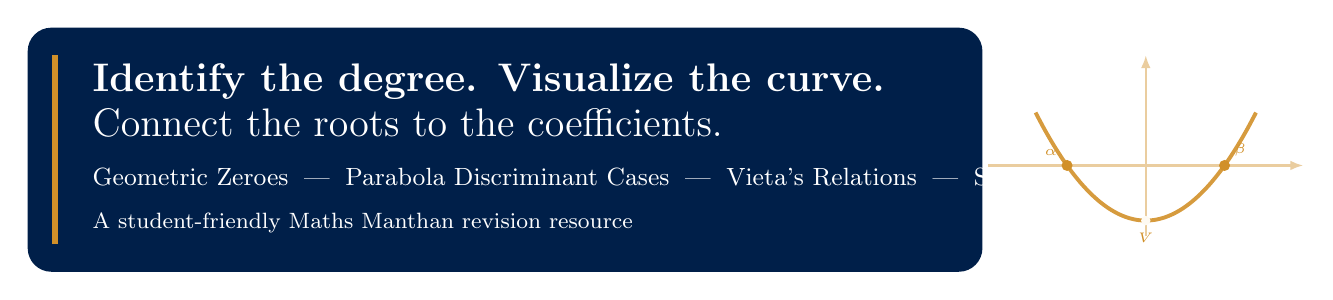
\begin{tikzpicture}
  \fill[navy,rounded corners=3mm] (0,0) rectangle (\textwidth,3.1);
  \draw[gold,line width=2pt] (0.35,0.35)--(0.35,2.75);
  \node[anchor=west,text=white,font=\bfseries\Large] at (0.7,2.42) {Identify the degree. Visualize the curve.};
  \node[anchor=west,text=white,font=\Large] at (0.7,1.90) {Connect the roots to the coefficients.};
  \node[anchor=west,text=white,font=\small] at (0.7,1.18) {Geometric Zeroes \;|\; Parabola Discriminant Cases \;|\; Vieta's Relations \;|\; Symmetric Functions};
  \node[anchor=west,text=white!75,font=\footnotesize] at (0.7,0.62) {A student-friendly Maths Manthan revision resource};
  
  % Stylized Parabola motif in gold
  \coordinate (Ograph) at (14.2, 1.35);
  \draw[gold!45, line width=0.8pt, -{Latex[scale=0.7]}] (12.2, 1.35) -- (16.2, 1.35);
  \draw[gold!45, line width=0.8pt, -{Latex[scale=0.7]}] (14.2, 0.45) -- (14.2, 2.75);
  \draw[gold!90, line width=1.4pt, domain=-1.4:1.4, smooth, variable=\x] 
    plot ({14.2 + \x}, {1.35 + 0.7*(\x*\x) - 0.7});
  \fill[gold] (14.2 - 1.0, 1.35) circle (0.07);
  \fill[gold] (14.2 + 1.0, 1.35) circle (0.07);
  \fill[accentlight] (14.2, 0.65) circle (0.06);
  \node[font=\tiny\bfseries\color{gold}, above left] at (14.2 - 1.0, 1.35) {$\alpha$};
  \node[font=\tiny\bfseries\color{gold}, above right] at (14.2 + 1.0, 1.35) {$\beta$};
  \node[font=\tiny\bfseries\color{gold}, below=1pt] at (14.2, 0.65) {$V$};
\end{tikzpicture}

\vspace{3mm}
\begin{minipage}[t]{0.48\textwidth}
  \begin{conceptBox}[title=What this handbook includes,fonttitle=\bfseries\color{navy}]
    \begin{itemize}
      \item Complete geometry of zeroes: Line and Parabola analysis.
      \item The 3 Discriminant cases ($D > 0, D = 0, D < 0$) in $6$ orientations.
      \item Vieta's formulas: $\alpha + \beta = -\frac{b}{a}$ and $\alpha\beta = \frac{c}{a}$.
      \item The 8 master symmetric identity expansions for board PYQs.
      \item Parameter conditions: Reciprocal, opposite, and ratio roots.
    \end{itemize}
  \end{conceptBox}
\end{minipage}\hfill
\begin{minipage}[t]{0.48\textwidth}
  \begin{formulaBox}[title=How to use this handbook,fonttitle=\bfseries\color{navy}]
    \raggedright Read the degree of the polynomial first. On graphs, count only the \textbf{intersections with the $x$-axis}. When forming quadratic polynomials, always include the non-zero real multiplier $k$ ($p(x) = k[x^2 - Sx + P]$) to clear denominators. Evaluate symmetric expressions using $S$ and $P$ directly without solving for roots.
  \end{formulaBox}
\end{minipage}

\vspace{1.5mm}
\begin{warningBox}[title=Official CBSE Curriculum Scope (Academic Year 2026--27),fonttitle=\bfseries\color{navy}]
  \textbf{Strict Syllabus Integrity \& Deleted Content:}
  Under the rationalized CBSE 2026--27 curriculum, the \textbf{Division Algorithm for Polynomials} ($p(x) = g(x)q(x) + r(x)$) and polynomial long division (former NCERT Exercise 2.3 and Exercise 2.4) have been \textbf{permanently excised} from Chapter 2. This handbook strictly covers the complete 100\% prescribed syllabus: Zeroes of polynomials, Geometrical meaning, and the Relationship between zeroes and coefficients of quadratic polynomials.
  {\scriptsize Source: \href{https://cbseacademic.nic.in/web_material/CurriculumMain27/SecPart1/Maths_SecP1X_2026-27.pdf}{CBSE Secondary Curriculum (2026--27), Unit II: Algebra}.}
\end{warningBox}

\vfill
\begin{center}
  {\small\bfseries\color{navy}Maths Manthan Tuition Classes}\\
  {\footnotesize\color{muted}contact@mathsmanthan.co.in \quad\textbar\quad +91-8171546558}\\
  {\footnotesize\url{https://mathsmanthan.co.in}}\\[2mm]
  {\scriptsize\color{muted}Prepared for learning and revision \;--\; not an official CBSE publication.}
\end{center}

\clearpage

% =============================================================================
% PAGE 2: MODULE 1 — ALGEBRAIC FOUNDATIONS & THE ANATOMY OF A POLYNOMIAL
% =============================================================================
\thispagestyle{fancy}
\vspace*{0mm}

\chapterbanner{02}{ALGEBRAIC FOUNDATIONS: POLYNOMIALS}{Definition, Classification by Degree and Terms \& Diagnostic Identification}{\SupportTag}

\subhead{Module 1.1 $\vert$ What is a Polynomial?}

An algebraic expression $p(x)$ in one variable $x$ is called a \textbf{polynomial} if all exponents of the variable $x$ are \textbf{non-negative integers} (whole numbers $\mathbb{W} = \{0, 1, 2, 3, \dots\}$):
\[
  \boxed{p(x) = a_n x^n + a_{n-1} x^{n-1} + a_{n-2} x^{n-2} + \dots + a_1 x + a_0}
\]
where $a_n, a_{n-1}, \dots, a_0 \in \mathbb{R}$ are real constants (coefficients) and $a_n \neq 0$. The highest exponent $n$ is the \textbf{Degree} of the polynomial.

\subhead{Module 1.2 $\vert$ The "Is It a Polynomial?" Diagnostic Test}

\begin{center}
\small
\begin{tabularx}{\textwidth}{>{\bfseries\color{navy}}p{28mm} c >{\color{secondary}}X}
\toprule
\rowcolor{bluepale}Expression & Polynomial? & Mathematical Reason \\
\midrule
$3x^2 - 5x + 7$ & \textbf{YES} & All exponents of $x$ are whole numbers ($2, 1, 0$). Coefficients are real. \\
$\sqrt{3}x^2 + \frac{1}{2}x$ & \textbf{YES} & Coefficients can be irrational or fractional. Powers of $x$ are integers ($2, 1$). \\
$2\sqrt{x} + 5$ & \textbf{NO} & Exponent of $x$ is fractional: $x^{1/2} \notin \mathbb{W}$. \\
$x^2 + \frac{3}{x} - 4$ & \textbf{NO} & Variable in denominator implies negative exponent: $x^{-1} \notin \mathbb{W}$. \\
$\frac{x^2 - 4}{x - 2}$ & \textbf{NO} & Rational expression with a domain restriction ($x \neq 2$). Not globally defined. \\
\bottomrule
\end{tabularx}
\end{center}

\vspace{-1mm}
\subhead{Module 1.3 $\vert$ Classification by Degree \& Term Count}

\begin{center}
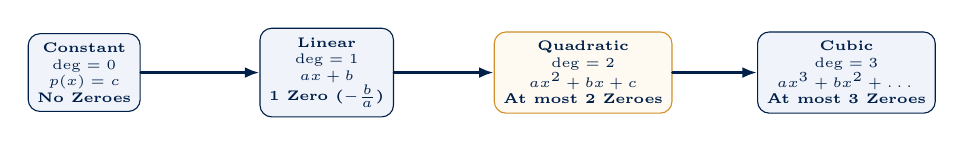
\begin{tikzpicture}[scale=0.88, line cap=round, line join=round]
  % Constant
  \node[draw=navy, fill=bluepale, rounded corners=1.5mm, font=\tiny\bfseries\color{navy}, align=center] (C0) at (0, 0) {
    \textbf{Constant}\\
    $\deg = 0$\\
    $p(x) = c$\\
    No Zeroes
  };
  % Linear
  \node[draw=navy, fill=bluepale, rounded corners=1.5mm, font=\tiny\bfseries\color{navy}, align=center] (C1) at (3.5, 0) {
    \textbf{Linear}\\
    $\deg = 1$\\
    $ax + b$\\
    1 Zero ($-\frac{b}{a}$)
  };
  % Quadratic
  \node[draw=accent, fill=accentlight, rounded corners=1.5mm, font=\tiny\bfseries\color{navy}, align=center] (C2) at (7.2, 0) {
    \textbf{Quadratic}\\
    $\deg = 2$\\
    $ax^2 + bx + c$\\
    At most 2 Zeroes
  };
  % Cubic
  \node[draw=navy, fill=bluepale, rounded corners=1.5mm, font=\tiny\bfseries\color{navy}, align=center] (C3) at (11.0, 0) {
    \textbf{Cubic}\\
    $\deg = 3$\\
    $ax^3 + bx^2 + \dots$\\
    At most 3 Zeroes
  };

  \draw[-{Latex[scale=0.7]}, primary, line width=1pt] (C0) -- (C1);
  \draw[-{Latex[scale=0.7]}, primary, line width=1pt] (C1) -- (C2);
  \draw[-{Latex[scale=0.7]}, primary, line width=1pt] (C2) -- (C3);
\end{tikzpicture}
\end{center}

\vspace{-2mm}
\subhead{Module 1.4 $\vert$ Value of a Polynomial $p(k)$ vs. Zero of a Polynomial}

\begin{formulaBox}
  \begin{itemize}
    \item \textbf{Value at $x = k$:} Obtained by substituting $x = k$ into $p(x)$, denoted as $p(k)$.
    \item \textbf{Zero of a Polynomial:} A real number $k$ is called a \textbf{zero} of $p(x)$ if and only if $\mathbf{p(k) = 0}$.
    \item \textbf{Fundamental Principle:} A polynomial of degree $n$ has \textbf{at most $n$ real zeroes}.
  \end{itemize}
\end{formulaBox}

\clearpage

% =============================================================================
% PAGE 3: MODULE 2 — GEOMETRIC MEANING OF ZEROES: THE PARABOLA ANATOMY
% =============================================================================
\thispagestyle{fancy}
\vspace*{0mm}

\chapterbanner{02}{GEOMETRIC MEANING OF ZEROES}{The Fundamental Coordinate Principle, Linear Lines \& Parabola Anatomy}{\CoreTag}

\subhead{Module 2.1 $\vert$ The Fundamental Coordinate-Geometry Principle}

\begin{formulaBox}
  The real zeroes of a polynomial $p(x)$ are precisely the \textbf{$x$-coordinates of the points where the graph of $y = p(x)$ intersects (or touches) the $x$-axis}.
  \[
    \boxed{p(k) = 0 \iff (k, 0) \in \text{Graph of } y = p(x)}
  \]
\end{formulaBox}

\subhead{Module 2.2 $\vert$ Graph of a Linear Polynomial ($y = ax + b, \; a \neq 0$)}

The graph of a linear polynomial is a straight line. Since a non-horizontal line intersects the $x$-axis at exactly one point, a linear polynomial has \textbf{exactly one zero}: $\mathbf{x = -\frac{b}{a}}$.

\subhead{Module 2.3 $\vert$ Graph of a Quadratic Polynomial ($y = ax^2 + bx + c$): The Parabola}

The graph of any quadratic polynomial is a continuous, U-shaped symmetrical curve called a \textbf{Parabola}.
\begin{itemize}
  \item \textbf{Orientation:} Opens \textbf{upward} ($\bigcup$) if $a > 0$; opens \textbf{downward} ($\bigcap$) if $a < 0$.
  \item \textbf{Axis of Symmetry:} The vertical line passing through the midpoint of the zeroes: $\mathbf{x = -\frac{b}{2a}}$.
  \item \textbf{Vertex ($V$):} The turning point (minimum when $a > 0$; maximum when $a < 0$): $\mathbf{V\left(-\frac{b}{2a}, -\frac{D}{4a}\right)}$.
  \item \textbf{$y$-Intercept:} Setting $x = 0$ gives $y = c$, so the graph always crosses the $y$-axis at $\mathbf{(0, c)}$.
\end{itemize}

\begin{center}
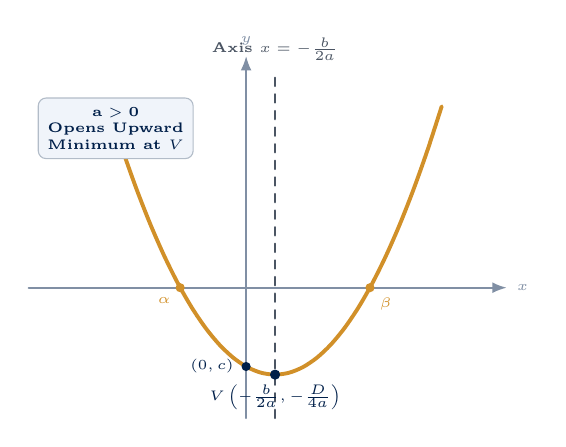
\begin{tikzpicture}[scale=0.92, line cap=round, line join=round]
  % Axes
  \draw[navy!50, line width=0.8pt, -{Latex[scale=0.8]}] (-3.0, 0) -- (3.6, 0) node[right, font=\tiny\bfseries]{$x$};
  \draw[navy!50, line width=0.8pt, -{Latex[scale=0.8]}] (0, -1.8) -- (0, 3.2) node[above, font=\tiny\bfseries]{$y$};

  % Upward Parabola: y = 0.7(x - 0.4)^2 - 1.2
  \draw[accent, line width=1.4pt, domain=-1.9:2.7, smooth, variable=\x] 
    plot ({\x}, {0.7*(\x - 0.4)*(\x - 0.4) - 1.2});

  % Axis of Symmetry
  \draw[secondary, line width=0.8pt, dashed] (0.4, -1.8) -- (0.4, 3.0) 
    node[above, font=\tiny\bfseries\color{secondary}]{Axis $x = -\frac{b}{2a}$};

  % Roots alpha and beta
  \fill[accent] (-0.91, 0) circle (1.8pt) node[below left, font=\tiny\bfseries\color{accent}]{$\alpha$};
  \fill[accent] (1.71, 0) circle (1.8pt) node[below right, font=\tiny\bfseries\color{accent}]{$\beta$};

  % Vertex V
  \fill[reddeep] (0.4, -1.2) circle (2pt) node[below, font=\tiny\bfseries\color{reddeep}]{$V\left(-\frac{b}{2a}, -\frac{D}{4a}\right)$};

  % y-intercept (0, c)
  \coordinate (Yint) at (0, {0.7*0.16 - 1.2});
  \fill[navy] (Yint) circle (1.8pt) node[left=1pt, font=\tiny\bfseries\color{navy}]{$(0, c)$};

  \node[draw=navy!30, fill=bluepale, rounded corners=1mm, font=\tiny\bfseries\color{navy}, align=center] at (-1.8, 2.2) {
    $\mathbf{a > 0}$\\
    Opens Upward\\
    Minimum at $V$
  };
\end{tikzpicture}
\end{center}

\vspace{-1mm}
\begin{conceptBox}[title=Geometric Core Rule: How Many Zeroes Does a Curve Have?,fonttitle=\bfseries\color{navy}]
  To determine the number of zeroes of any polynomial from its graph, count the number of times the curve \textbf{cuts or touches the $x$-axis}. Intersections with the $y$-axis are irrelevant to zeroes!
\end{conceptBox}

\clearpage

% =============================================================================
% PAGE 4: MODULE 3 — THE THREE DISCRIMINANT CASES & GRAPH READING PROTOCOLS
% =============================================================================
\thispagestyle{fancy}
\vspace*{0mm}

\chapterbanner{02}{THE THREE DISCRIMINANT CASES}{The 6-Parabola Matrix, Intersections vs. Contacts \& Graph Reading Protocols}{\CoreTag}

\subhead{Module 3.1 $\vert$ The Discriminant ($D = b^2 - 4ac$) as the Geometric Arbiter}

The sign of the discriminant $D = b^2 - 4ac$ uniquely determines how many times the parabola meets the $x$-axis:

\begin{center}
\small
\begin{tabularx}{\textwidth}{c >{\bfseries\color{navy}}p{22mm} c c X}
\toprule
\rowcolor{bluepale}Case & Discriminant & Common Points & Real Zeroes & Geometric Behavior of Parabola \\
\midrule
I & $\mathbf{D > 0}$ & $2$ & $2$ distinct & Parabola cuts cleanly through $x$-axis at $(\alpha, 0)$ and $(\beta, 0)$. \\
II & $\mathbf{D = 0}$ & $1$ (tangent) & $1$ repeated & Parabola touches the $x$-axis at its vertex $V\left(-\frac{b}{2a}, 0\right)$. \\
III & $\mathbf{D < 0}$ & $0$ & $0$ real & Parabola does not meet $x$-axis at all (lies entirely above or below). \\
\bottomrule
\end{tabularx}
\end{center}

\vspace{-1mm}
\subhead{Module 3.2 $\vert$ The Six-Parabola Matrix}

\begin{center}
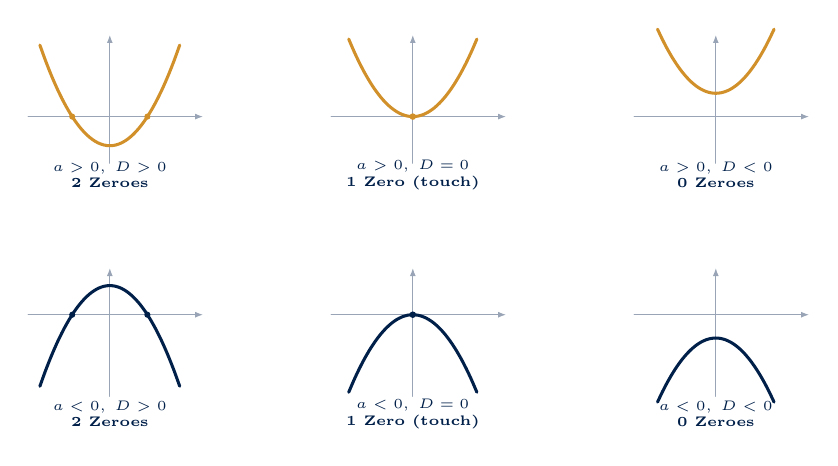
\begin{tikzpicture}[scale=0.74, line cap=round, line join=round]
  % Row 1: a > 0 (Upward)
  % D > 0
  \begin{scope}[shift={(0,2.6)}]
    \draw[navy!40, -{Latex[scale=0.6]}] (-1.4,0) -- (1.6,0);
    \draw[navy!40, -{Latex[scale=0.6]}] (0,-0.8) -- (0,1.4);
    \draw[accent, line width=1.1pt, domain=-1.2:1.2, smooth] plot ({\x}, {1.2*\x*\x - 0.5});
    \fill[accent] (-0.645,0) circle (1.5pt); \fill[accent] (0.645,0) circle (1.5pt);
    \node[font=\tiny\bfseries\color{navy}, align=center] at (0,-1.0) {$a>0, \; D>0$\\\textbf{2 Zeroes}};
  \end{scope}

  % D = 0
  \begin{scope}[shift={(5.2,2.6)}]
    \draw[navy!40, -{Latex[scale=0.6]}] (-1.4,0) -- (1.6,0);
    \draw[navy!40, -{Latex[scale=0.6]}] (0,-0.8) -- (0,1.4);
    \draw[accent, line width=1.1pt, domain=-1.1:1.1, smooth] plot ({\x}, {1.1*\x*\x});
    \fill[accent] (0,0) circle (1.6pt);
    \node[font=\tiny\bfseries\color{navy}, align=center] at (0,-1.0) {$a>0, \; D=0$\\\textbf{1 Zero (touch)}};
  \end{scope}

  % D < 0
  \begin{scope}[shift={(10.4,2.6)}]
    \draw[navy!40, -{Latex[scale=0.6]}] (-1.4,0) -- (1.6,0);
    \draw[navy!40, -{Latex[scale=0.6]}] (0,-0.8) -- (0,1.4);
    \draw[accent, line width=1.1pt, domain=-1.0:1.0, smooth] plot ({\x}, {1.1*\x*\x + 0.4});
    \node[font=\tiny\bfseries\color{navy}, align=center] at (0,-1.0) {$a>0, \; D<0$\\\textbf{0 Zeroes}};
  \end{scope}

  % Row 2: a < 0 (Downward)
  % D > 0
  \begin{scope}[shift={(0,-0.8)}]
    \draw[navy!40, -{Latex[scale=0.6]}] (-1.4,0) -- (1.6,0);
    \draw[navy!40, -{Latex[scale=0.6]}] (0,-1.4) -- (0,0.8);
    \draw[reddeep, line width=1.1pt, domain=-1.2:1.2, smooth] plot ({\x}, {-1.2*\x*\x + 0.5});
    \fill[reddeep] (-0.645,0) circle (1.5pt); \fill[reddeep] (0.645,0) circle (1.5pt);
    \node[font=\tiny\bfseries\color{navy}, align=center] at (0,-1.7) {$a<0, \; D>0$\\\textbf{2 Zeroes}};
  \end{scope}

  % D = 0
  \begin{scope}[shift={(5.2,-0.8)}]
    \draw[navy!40, -{Latex[scale=0.6]}] (-1.4,0) -- (1.6,0);
    \draw[navy!40, -{Latex[scale=0.6]}] (0,-1.4) -- (0,0.8);
    \draw[reddeep, line width=1.1pt, domain=-1.1:1.1, smooth] plot ({\x}, {-1.1*\x*\x});
    \fill[reddeep] (0,0) circle (1.6pt);
    \node[font=\tiny\bfseries\color{navy}, align=center] at (0,-1.7) {$a<0, \; D=0$\\\textbf{1 Zero (touch)}};
  \end{scope}

  % D < 0
  \begin{scope}[shift={(10.4,-0.8)}]
    \draw[navy!40, -{Latex[scale=0.6]}] (-1.4,0) -- (1.6,0);
    \draw[navy!40, -{Latex[scale=0.6]}] (0,-1.4) -- (0,0.8);
    \draw[reddeep, line width=1.1pt, domain=-1.0:1.0, smooth] plot ({\x}, {-1.1*\x*\x - 0.4});
    \node[font=\tiny\bfseries\color{navy}, align=center] at (0,-1.7) {$a<0, \; D<0$\\\textbf{0 Zeroes}};
  \end{scope}
\end{tikzpicture}
\end{center}

\vspace{-1mm}
\subhead{Module 3.3 $\vert$ NCERT Exercise 2.1 Graph-Reading Protocol}

\begin{warningBox}[title=Board Exam 1-Mark MCQ Protocol: Reading Curves,fonttitle=\bfseries\color{reddeep}]
  When a question asks \textit{"Find the number of zeroes of $y = p(x)$ from the given figure"}:
  \begin{enumerate}[itemsep=1pt]
    \item Focus \textbf{exclusively on the horizontal $x$-axis}. Ignore where the curve intersects the $y$-axis.
    \item Each distinct crossing counts as 1 zero. Each point of tangency (touching without crossing) counts as 1 repeated real zero.
    \item If the curve does not meet the $x$-axis, write: \textbf{"Number of zeroes = 0"}.
  \end{enumerate}
\end{warningBox}

\clearpage

% =============================================================================
% PAGE 5: MODULE 4 — QUADRATIC ZEROES & COEFFICIENTS: VIETA'S RELATIONS
% =============================================================================
\thispagestyle{fancy}
\vspace*{0mm}

\chapterbanner{02}{ZEROES \& COEFFICIENTS: VIETA'S RELATIONS}{Factor Theorem Derivation, Verification Protocols \& Parabola Symmetry}{\CoreTag}

\subhead{Module 4.1 $\vert$ Factor Theorem Derivation of Vieta's Relations}

Let $p(x) = ax^2 + bx + c$ ($a \neq 0$) have two real zeroes $\alpha$ and $\beta$.
By the \textbf{Factor Theorem}, $(x - \alpha)$ and $(x - \beta)$ are factors of $p(x)$:
\[
  ax^2 + bx + c = k(x - \alpha)(x - \beta) = k\left[x^2 - (\alpha + \beta)x + \alpha\beta\right] = kx^2 - k(\alpha + \beta)x + k\alpha\beta
\]
Equating coefficients of like powers of $x$:
\[
  a = k, \qquad b = -a(\alpha + \beta) \implies \mathbf{\alpha + \beta = -\frac{b}{a}}, \qquad c = a\alpha\beta \implies \mathbf{\alpha\beta = \frac{c}{a}}
\]

\begin{formulaBox}
  \[
    \boxed{\mathbf{S = \alpha + \beta = -\frac{b}{a} = -\frac{\text{Coeff.\ of } x}{\text{Coeff.\ of } x^2}}}
    \qquad
    \boxed{\mathbf{P = \alpha\beta = \frac{c}{a} = \frac{\text{Constant term}}{\text{Coeff.\ of } x^2}}}
  \]
\end{formulaBox}

\subhead{Module 4.2 $\vert$ Geometric Interpretation: The Symmetry of Roots}

\begin{minipage}[t]{0.58\textwidth}
  Notice that the axis of symmetry of the parabola $y = ax^2 + bx + c$ is located at the exact arithmetic midpoint of the two zeroes:
  \[
    x_{\text{mid}} = \frac{\alpha + \beta}{2} = \frac{-\frac{b}{a}}{2} = \mathbf{-\frac{b}{2a}}
  \]
  Thus, Vieta's sum of zeroes is directly encoded as the horizontal location of the parabola's vertex!
\end{minipage}\hfill
\begin{minipage}[t]{0.39\textwidth}
  \begin{center}
  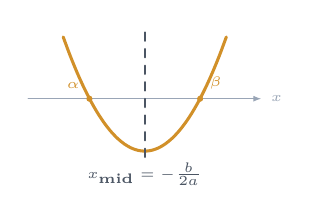
\begin{tikzpicture}[scale=0.74, line cap=round, line join=round]
    \draw[navy!40, -{Latex[scale=0.6]}] (-2.0,0) -- (2.0,0) node[right, font=\tiny\bfseries]{$x$};
    \draw[accent, line width=1.1pt, domain=-1.4:1.4, smooth] plot ({\x}, {\x*\x - 0.9});
    \draw[secondary, line width=0.8pt, dashed] (0,-1.0) -- (0,1.2);
    \fill[accent] (-0.95,0) circle (1.5pt) node[above left, font=\tiny\bfseries]{$\alpha$};
    \fill[accent] (0.95,0) circle (1.5pt) node[above right, font=\tiny\bfseries]{$\beta$};
    \node[font=\tiny\bfseries\color{secondary}, align=center] at (0,-1.3) {$x_{\text{mid}} = -\frac{b}{2a}$};
  \end{tikzpicture}
  \end{center}
\end{minipage}

\vspace{-1mm}
\subhead{Module 4.3 $\vert$ Worked Archetype 1: Finding Zeroes \& Verifying Relations}

\begin{conceptBox}[title=Worked Archetype 1: Complete CBSE Board 3-Marker Protocol,fonttitle=\bfseries\color{navy}]
  \textbf{Problem:} Find zeroes of $p(x) = 6x^2 - 3 - 7x$ and verify relations with coefficients.\\
  \textbf{Solution:}
  \begin{enumerate}[leftmargin=4.5mm, itemsep=1pt]
    \item \textbf{Standard Form:} $p(x) = 6x^2 - 7x - 3$. Here $a = 6, b = -7, c = -3$.
    \item \textbf{Factorization:} $6x^2 - 9x + 2x - 3 = 3x(2x - 3) + 1(2x - 3) = (2x - 3)(3x + 1)$.
    \item Zeroes: $2x - 3 = 0 \implies \mathbf{\alpha = \frac{3}{2}}$ \quad and \quad $3x + 1 = 0 \implies \mathbf{\beta = -\frac{1}{3}}$.
    \item \textbf{Verification:}
      $\alpha + \beta = \frac{3}{2} - \frac{1}{3} = \frac{7}{6}$ and $-\frac{b}{a} = -\frac{-7}{6} = \frac{7}{6}$ [Verified].\\
      $\alpha\beta = \left(\frac{3}{2}\right)\left(-\frac{1}{3}\right) = -\frac{1}{2}$ and $\frac{c}{a} = \frac{-3}{6} = -\frac{1}{2}$ [Verified].
  \end{enumerate}
\end{conceptBox}

\clearpage

% =============================================================================
% PAGE 6: MODULE 5 — FORMATION OF QUADRATIC POLYNOMIALS
% =============================================================================
\thispagestyle{fancy}
\vspace*{0mm}

\chapterbanner{02}{FORMATION OF QUADRATIC POLYNOMIALS}{Reconstructing Polynomials from Zeroes \& The Vital Role of Constant $k$}{\CoreTag}

\subhead{Module 5.1 $\vert$ The General Reconstruction Formula}

If $\alpha$ and $\beta$ are the zeroes of a quadratic polynomial, the polynomial can be reconstructed uniquely up to a non-zero scaling factor $k$:

\begin{formulaBox}
  \[
    \boxed{p(x) = k\left[x^2 - (\alpha + \beta)x + \alpha\beta\right] = \mathbf{k\left[x^2 - S x + P\right]}}
  \]
  where $S = \alpha + \beta$ is the \textbf{Sum}, $P = \alpha\beta$ is the \textbf{Product}, and $k \in \mathbb{R} \setminus \{0\}$.
\end{formulaBox}

\subhead{Module 5.2 $\vert$ Why the Constant $k$ is Mandatory: The Family of Polynomials}

A pair of zeroes does not specify a single unique polynomial, but an \textbf{infinite family of scaled polynomials} having identical $x$-intercepts:

\begin{minipage}[t]{0.56\textwidth}
  \textbf{Example with Fractional Coefficients:} \\
  Suppose $S = -\frac{1}{4}$ and $P = \frac{1}{4}$.
  \[
    p(x) = k\left[x^2 - \left(-\frac{1}{4}\right)x + \frac{1}{4}\right] = k\left[x^2 + \frac{1}{4}x + \frac{1}{4}\right]
  \]
  \begin{itemize}[itemsep=1pt]
    \item Setting $k = 4$ clears the fractions to give integer coefficients:
      \[
        \mathbf{p(x) = 4x^2 + x + 1}
      \]
    \item Both $x^2 + \frac{1}{4}x + \frac{1}{4}$ and $4x^2 + x + 1$ share the exact same zeroes!
  \end{itemize}
\end{minipage}\hfill
\begin{minipage}[t]{0.41\textwidth}
  \begin{center}
  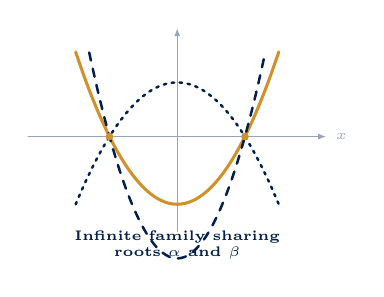
\begin{tikzpicture}[scale=0.86, line cap=round, line join=round]
    \draw[navy!40, -{Latex[scale=0.6]}] (-2.2,0) -- (2.2,0) node[right, font=\tiny\bfseries]{$x$};
    \draw[navy!40, -{Latex[scale=0.6]}] (0,-1.4) -- (0,1.6);
    \draw[accent, line width=1.1pt, domain=-1.5:1.5, smooth] plot ({\x}, {\x*\x - 1.0});
    \draw[primary, line width=0.9pt, dashed, domain=-1.3:1.3, smooth] plot ({\x}, {1.8*(\x*\x - 1.0)});
    \draw[reddeep, line width=0.9pt, dotted, domain=-1.5:1.5, smooth] plot ({\x}, {-0.8*(\x*\x - 1.0)});
    \fill[accent] (-1.0,0) circle (1.6pt); \fill[accent] (1.0,0) circle (1.6pt);
    \node[font=\tiny\bfseries\color{navy}, align=center] at (0,-1.6) {Infinite family sharing\\roots $\alpha$ and $\beta$};
  \end{tikzpicture}
  \end{center}
\end{minipage}

\vspace{-1mm}
\subhead{Module 5.3 $\vert$ Worked Archetypes: Forming Quadratic Polynomials}

\begin{conceptBox}[title=Worked Archetype 2: Given Zeroes vs. Given Sum and Product,fonttitle=\bfseries\color{navy}]
  \textbf{Case A (Direct Sum and Product):} Find a quadratic polynomial with sum $S = \sqrt{2}$ and product $P = \frac{1}{3}$.\\
  \textbf{Solution:} $p(x) = k\left[x^2 - Sx + P\right] = k\left[x^2 - \sqrt{2}x + \frac{1}{3}\right]$. Setting $k = 3$: $\mathbf{p(x) = 3x^2 - 3\sqrt{2}x + 1}$.

  \vspace{1mm}
  \textbf{Case B (Individual Zeroes Given):} Find a quadratic polynomial whose zeroes are $2 + \sqrt{3}$ and $2 - \sqrt{3}$.\\
  \textbf{Solution:}
  \begin{itemize}[itemsep=1pt]
    \item $S = (2 + \sqrt{3}) + (2 - \sqrt{3}) = 4$.
    \item $P = (2 + \sqrt{3})(2 - \sqrt{3}) = 2^2 - (\sqrt{3})^2 = 4 - 3 = 1$.
    \item $p(x) = k[x^2 - 4x + 1]$. For $k = 1$: $\mathbf{p(x) = x^2 - 4x + 1}$.
  \end{itemize}
\end{conceptBox}

\clearpage

% =============================================================================
% PAGE 7: MODULE 6 — MASTER TOOLKIT: SYMMETRIC FUNCTIONS OF ZEROES
% =============================================================================
\thispagestyle{fancy}
\vspace*{0mm}

\chapterbanner{02}{SYMMETRIC FUNCTIONS OF ZEROES}{The 8 Core Algebraic Transformations \& Identity Derivations in $S$ and $P$}{\CoreTag}

\subhead{Module 6.1 $\vert$ The Principle of Symmetric Functions}

An algebraic expression in $\alpha$ and $\beta$ is called \textbf{symmetric} if swapping $\alpha$ and $\beta$ leaves the expression unchanged ($f(\alpha, \beta) = f(\beta, \alpha)$). \\
\textbf{The Golden Rule of Board Evaluation:} Never calculate $\alpha$ and $\beta$ individually! Express symmetric functions strictly in terms of $\mathbf{S = \alpha + \beta = -\frac{b}{a}}$ and $\mathbf{P = \alpha\beta = \frac{c}{a}}$.

\subhead{Module 6.2 $\vert$ The 8 Essential Algebraic Identities}

\begin{center}
\small
\begin{tabularx}{\textwidth}{c >{\bfseries\color{navy}}p{32mm} >{\bfseries\color{primary}}p{42mm} X}
\toprule
\rowcolor{bluepale}\# & Expression & Identity in $S$ and $P$ & Derivation / Expansion Blueprint \\
\midrule
1 & $\mathbf{\alpha^2 + \beta^2}$ & $\mathbf{S^2 - 2P}$ & From $(\alpha+\beta)^2 = \alpha^2 + \beta^2 + 2\alpha\beta$. \\
2 & $\mathbf{\frac{1}{\alpha} + \frac{1}{\beta}}$ & $\mathbf{\frac{S}{P}}$ & Take common denominator: $\frac{\beta+\alpha}{\alpha\beta} = \frac{S}{P}$. \\
3 & $\mathbf{\frac{\alpha}{\beta} + \frac{\beta}{\alpha}}$ & $\mathbf{\frac{S^2 - 2P}{P}}$ & Combine: $\frac{\alpha^2+\beta^2}{\alpha\beta} = \frac{S^2 - 2P}{P}$. \\
4 & $\mathbf{(\alpha - \beta)^2}$ & $\mathbf{S^2 - 4P}$ & $(\alpha+\beta)^2 - 4\alpha\beta = S^2 - 4P \implies |\alpha - \beta| = \sqrt{S^2 - 4P}$. \\
5 & $\mathbf{\alpha^3 + \beta^3}$ & $\mathbf{S^3 - 3SP}$ & From $(\alpha+\beta)^3 = \alpha^3 + \beta^3 + 3\alpha\beta(\alpha+\beta)$. \\
6 & $\mathbf{\alpha^2\beta + \alpha\beta^2}$ & $\mathbf{PS}$ & Factor out product: $\alpha\beta(\alpha+\beta) = P \cdot S$. \\
7 & $\mathbf{\frac{1}{\alpha^2} + \frac{1}{\beta^2}}$ & $\mathbf{\frac{S^2 - 2P}{P^2}}$ & $\frac{\alpha^2+\beta^2}{(\alpha\beta)^2} = \frac{S^2 - 2P}{P^2}$. \\
8 & $\mathbf{\alpha^4 + \beta^4}$ & $\mathbf{(S^2 - 2P)^2 - 2P^2}$ & Treat as $(\alpha^2+\beta^2)^2 - 2(\alpha\beta)^2$. \\
\bottomrule
\end{tabularx}
\end{center}

\vspace{-1mm}
\subhead{Module 6.3 $\vert$ The Symmetric Function Architecture}

\begin{center}
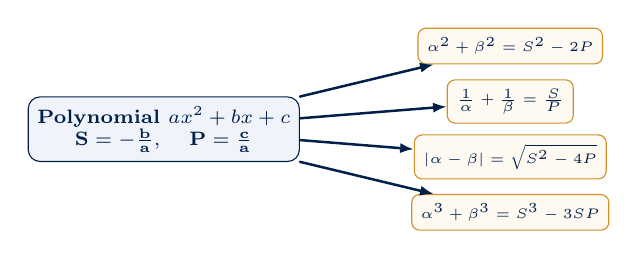
\begin{tikzpicture}[scale=0.88, line cap=round, line join=round]
  % Input Box
  \node[draw=navy, fill=bluepale, rounded corners=1.5mm, font=\scriptsize\bfseries\color{navy}, align=center] (Inputs) at (0, 0) {
    Polynomial $ax^2 + bx + c$\\
    $\mathbf{S = -\frac{b}{a}}, \quad \mathbf{P = \frac{c}{a}}$
  };

  % Outputs
  \node[draw=accent, fill=accentlight, rounded corners=1mm, font=\tiny\bfseries\color{navy}] (O1) at (5.0, 1.2) {$\alpha^2 + \beta^2 = S^2 - 2P$};
  \node[draw=accent, fill=accentlight, rounded corners=1mm, font=\tiny\bfseries\color{navy}] (O2) at (5.0, 0.4) {$\frac{1}{\alpha} + \frac{1}{\beta} = \frac{S}{P}$};
  \node[draw=accent, fill=accentlight, rounded corners=1mm, font=\tiny\bfseries\color{navy}] (O3) at (5.0, -0.4) {$|\alpha - \beta| = \sqrt{S^2 - 4P}$};
  \node[draw=accent, fill=accentlight, rounded corners=1mm, font=\tiny\bfseries\color{navy}] (O4) at (5.0, -1.2) {$\alpha^3 + \beta^3 = S^3 - 3SP$};

  \draw[-{Latex[scale=0.7]}, primary, line width=0.9pt] (Inputs) -- (O1);
  \draw[-{Latex[scale=0.7]}, primary, line width=0.9pt] (Inputs) -- (O2);
  \draw[-{Latex[scale=0.7]}, primary, line width=0.9pt] (Inputs) -- (O3);
  \draw[-{Latex[scale=0.7]}, primary, line width=0.9pt] (Inputs) -- (O4);
\end{tikzpicture}
\end{center}

\clearpage

% =============================================================================
% PAGE 8: MODULE 7 — WORKED BOARD-EXAM MASTER MODELS
% =============================================================================
\thispagestyle{fancy}
\vspace*{0mm}

\chapterbanner{02}{WORKED BOARD-EXAM MASTER MODELS}{Expression Evaluations, Root Transformations \& Finding Unknown Parameters}{\WorkedTag}

\subhead{Module 7.1 $\vert$ Master Model 1: Non-Factorable Expression Evaluation}

\begin{conceptBox}[title=Worked Archetype 3: Evaluating Complex Symmetric Expressions,fonttitle=\bfseries\color{navy}]
  \textbf{Problem:} If $\alpha$ and $\beta$ are the zeroes of $p(x) = 2x^2 - 5x + 7$, find the value of: (i) $\frac{1}{\alpha} + \frac{1}{\beta}$ \quad (ii) $\alpha^3 + \beta^3$.\\
  \textbf{Solution:}
  Here $a = 2, b = -5, c = 7$.
  $S = \alpha + \beta = -\frac{-5}{2} = \frac{5}{2}$, \quad $P = \alpha\beta = \frac{7}{2}$.
  \begin{enumerate}[leftmargin=4.5mm, itemsep=1.5pt]
    \item $\frac{1}{\alpha} + \frac{1}{\beta} = \frac{\alpha+\beta}{\alpha\beta} = \frac{\frac{5}{2}}{\frac{7}{2}} = \mathbf{\frac{5}{7}}$.
    \item $\alpha^3 + \beta^3 = (\alpha+\beta)^3 - 3\alpha\beta(\alpha+\beta) = \left(\frac{5}{2}\right)^3 - 3\left(\frac{7}{2}\right)\left(\frac{5}{2}\right) = \frac{125}{8} - \frac{105}{4} = \frac{125 - 210}{8} = \mathbf{-\frac{85}{8}}$.
  \end{enumerate}
\end{conceptBox}

\subhead{Module 7.2 $\vert$ Master Model 2: Forming Polynomials with Transformed Zeroes}

\begin{conceptBox}[title=Worked Archetype 4: Polynomial with Reciprocal Zeroes,fonttitle=\bfseries\color{navy}]
  \textbf{Problem:} If $\alpha, \beta$ are zeroes of $p(x) = x^2 - 2x - 15$, form a quadratic polynomial whose zeroes are $\frac{1}{\alpha}$ and $\frac{1}{\beta}$.\\
  \textbf{Solution:}
  For $p(x)$, $\alpha + \beta = 2$ and $\alpha\beta = -15$.
  Let $S'$ and $P'$ be the sum and product of the new zeroes:
  \begin{itemize}[itemsep=1pt]
    \item $S' = \frac{1}{\alpha} + \frac{1}{\beta} = \frac{\alpha+\beta}{\alpha\beta} = \frac{2}{-15} = -\frac{2}{15}$.
    \item $P' = \frac{1}{\alpha} \cdot \frac{1}{\beta} = \frac{1}{\alpha\beta} = -\frac{1}{15}$.
    \item Required polynomial: $q(x) = k[x^2 - S'x + P'] = k\left[x^2 - \left(-\frac{2}{15}\right)x + \left(-\frac{1}{15}\right)\right] = k\left[x^2 + \frac{2}{15}x - \frac{1}{15}\right]$.
    \item Setting $k = 15$ gives: $\mathbf{q(x) = 15x^2 + 2x - 1}$.
  \end{itemize}
\end{conceptBox}

\subhead{Module 7.3 $\vert$ Master Model 3: Finding Unknown Parameter $k$}

\begin{conceptBox}[title=Worked Archetype 5: Parameter with Zero-Difference Condition,fonttitle=\bfseries\color{navy}]
  \textbf{Problem:} If the zeroes of $p(x) = x^2 - 8x + k$ satisfy $(\alpha - \beta) = 2$, find the value of $k$.\\
  \textbf{Solution:}
  Here $a = 1, b = -8, c = k \implies \alpha + \beta = 8$ and $\alpha\beta = k$.
  Using identity: $(\alpha - \beta)^2 = (\alpha + \beta)^2 - 4\alpha\beta$:
  \[
    (2)^2 = (8)^2 - 4k \implies 4 = 64 - 4k \implies 4k = 60 \implies \mathbf{k = 15}.
  \]
\end{conceptBox}

\clearpage

% =============================================================================
% PAGE 9: MODULE 8 — SPECIAL ZERO CONFIGURATIONS
% =============================================================================
\thispagestyle{fancy}
\vspace*{0mm}

\chapterbanner{02}{SPECIAL ZERO CONFIGURATIONS}{Reciprocal Roots, Additive Inverses \& Rapid Elimination Shortcuts}{\WorkedTag}

\subhead{Module 8.1 $\vert$ Reciprocal Zeroes Theorem ($\beta = \frac{1}{\alpha}$)}

\begin{formulaBox}
  If one zero of $p(x) = ax^2 + bx + c$ is the \textbf{reciprocal} of the other:
  \[
    \alpha \cdot \beta = 1 \implies \frac{c}{a} = 1 \implies \mathbf{c = a}
  \]
  \textbf{Board Shortcut:} Whenever a question states "one zero is reciprocal of the other", directly equate $\mathbf{\text{Constant term} = \text{Coefficient of } x^2}$.
\end{formulaBox}

\subhead{Module 8.2 $\vert$ Equal and Opposite Zeroes Theorem ($\beta = -\alpha$)}

\begin{formulaBox}
  If one zero is the \textbf{negative (additive inverse)} of the other:
  \[
    \alpha + \beta = 0 \implies -\frac{b}{a} = 0 \implies \mathbf{b = 0}
  \]
  \textbf{Geometric Implication:} When $b = 0$, the axis of symmetry is $x = 0$ (the $y$-axis). The parabola is perfectly symmetric about the $y$-axis!
\end{formulaBox}

\begin{center}
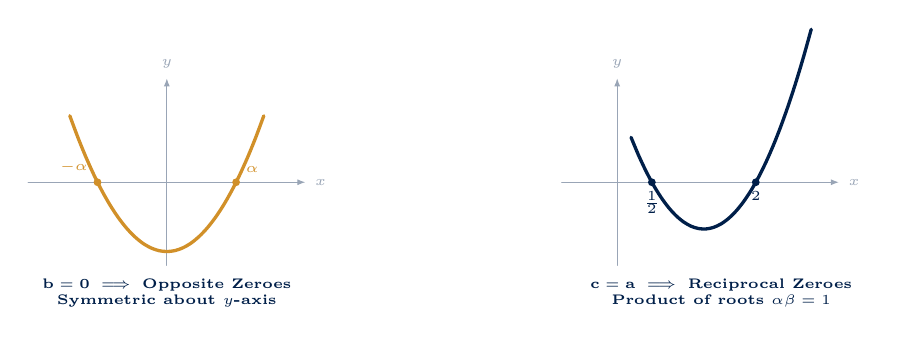
\begin{tikzpicture}[scale=0.88, line cap=round, line join=round]
  % b = 0 Parabola
  \begin{scope}[shift={(0,0)}]
    \draw[navy!40, -{Latex[scale=0.6]}] (-2.0,0) -- (2.0,0) node[right, font=\tiny\bfseries]{$x$};
    \draw[navy!40, -{Latex[scale=0.6]}] (0,-1.2) -- (0,1.5) node[above, font=\tiny\bfseries]{$y$};
    \draw[accent, line width=1.2pt, domain=-1.4:1.4, smooth] plot ({\x}, {\x*\x - 1.0});
    \fill[accent] (-1.0,0) circle (1.6pt) node[above left, font=\tiny\bfseries]{$-\alpha$};
    \fill[accent] (1.0,0) circle (1.6pt) node[above right, font=\tiny\bfseries]{$\alpha$};
    \node[font=\tiny\bfseries\color{navy}, align=center] at (0,-1.6) {$\mathbf{b = 0} \implies \text{Opposite Zeroes}$\\Symmetric about $y$-axis};
  \end{scope}

  % c = a Parabola
  \begin{scope}[shift={(6.5,0)}]
    \draw[navy!40, -{Latex[scale=0.6]}] (-0.8,0) -- (3.2,0) node[right, font=\tiny\bfseries]{$x$};
    \draw[navy!40, -{Latex[scale=0.6]}] (0,-1.2) -- (0,1.5) node[above, font=\tiny\bfseries]{$y$};
    \draw[primary, line width=1.2pt, domain=0.2:2.8, smooth] plot ({\x}, {1.2*(\x - 0.5)*(\x - 2.0)});
    \fill[primary] (0.5,0) circle (1.6pt) node[below, font=\tiny\bfseries]{$\frac{1}{2}$};
    \fill[primary] (2.0,0) circle (1.6pt) node[below, font=\tiny\bfseries]{$2$};
    \node[font=\tiny\bfseries\color{navy}, align=center] at (1.5,-1.6) {$\mathbf{c = a} \implies \text{Reciprocal Zeroes}$\\Product of roots $\alpha\beta = 1$};
  \end{scope}
\end{tikzpicture}
\end{center}

\vspace{-1mm}
\subhead{Module 8.3 $\vert$ Zeroes in a Given Ratio ($\alpha : \beta = m : n$)}

\begin{formulaBox}
  If the zeroes of $ax^2 + bx + c$ are in the ratio $m : n$, then:
  \[
    \boxed{\frac{(m + n)^2}{mn} = \frac{b^2}{ac}}
  \]
  \textit{Proof:} Let $\alpha = mk, \beta = nk$. Then $\alpha + \beta = (m+n)k = -\frac{b}{a}$ and $\alpha\beta = mn k^2 = \frac{c}{a}$. Dividing $(S)^2$ by $P$ immediately yields the identity.
\end{formulaBox}

\clearpage

% =============================================================================
% PAGE 10: MODULE 9 — ENRICHMENT BRIDGE: CUBIC POLYNOMIALS
% =============================================================================
\thispagestyle{fancy}
\vspace*{0mm}

\chapterbanner{02}{ENRICHMENT BRIDGE: CUBIC POLYNOMIALS}{Higher-Degree Vieta Relations, Cubic Curve Geometry \& Syllabus Demarcation}{\ExtensionTag}

\subhead{Module 9.1 $\vert$ Vieta's Relations for Cubic Polynomials}

A cubic polynomial has degree $3$ and at most $3$ real zeroes:
\[
  p(x) = ax^3 + bx^2 + cx + d \quad (a \neq 0)
\]
If $\alpha, \beta, \gamma$ are the zeroes of $p(x)$, then $p(x) = k(x - \alpha)(x - \beta)(x - \gamma)$. Expanding and equating coefficients yields:

\begin{formulaBox}
  \begin{align*}
    \textbf{Sum of Zeroes: } & \mathbf{\alpha + \beta + \gamma = -\frac{b}{a}} = -\frac{\text{coeff. of } x^2}{\text{coeff. of } x^3} \\
    \textbf{Sum of Products taken two at a time: } & \mathbf{\alpha\beta + \beta\gamma + \gamma\alpha = \frac{c}{a}} = \frac{\text{coeff. of } x}{\text{coeff. of } x^3} \\
    \textbf{Product of all three Zeroes: } & \mathbf{\alpha\beta\gamma = -\frac{d}{a}} = -\frac{\text{constant term}}{\text{coeff. of } x^3}
  \end{align*}
\end{formulaBox}

\subhead{Module 9.2 $\vert$ Geometric Behavior of a Cubic Polynomial}

\begin{minipage}[t]{0.56\textwidth}
  The graph of a cubic polynomial is an S-shaped curve that can intersect the $x$-axis at $1, 2$, or $3$ points.
  \begin{itemize}[itemsep=1pt]
    \item A cubic polynomial always has \textbf{at least one real zero} (complex roots occur in conjugate pairs).
    \item Formation:
      \[
        \mathbf{p(x) = k\left[x^3 - S_1 x^2 + S_2 x - S_3\right]}
      \]
      where $S_1 = \sum\alpha, \; S_2 = \sum\alpha\beta, \; S_3 = \alpha\beta\gamma$.
  \end{itemize}
\end{minipage}\hfill
\begin{minipage}[t]{0.41\textwidth}
  \begin{center}
  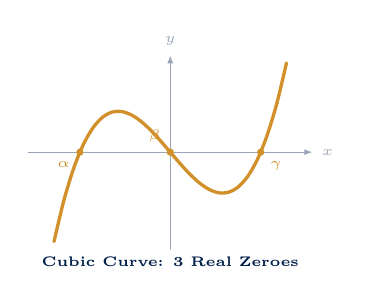
\begin{tikzpicture}[scale=0.82, line cap=round, line join=round]
    \draw[navy!40, -{Latex[scale=0.6]}] (-2.2,0) -- (2.2,0) node[right, font=\tiny\bfseries]{$x$};
    \draw[navy!40, -{Latex[scale=0.6]}] (0,-1.5) -- (0,1.5) node[above, font=\tiny\bfseries]{$y$};
    \draw[accent, line width=1.2pt, domain=-1.8:1.8, smooth] plot ({\x}, {0.6*\x*(\x*\x - 1.96)});
    \fill[accent] (-1.4,0) circle (1.6pt) node[below left, font=\tiny\bfseries]{$\alpha$};
    \fill[accent] (0,0) circle (1.6pt) node[above left, font=\tiny\bfseries]{$\beta$};
    \fill[accent] (1.4,0) circle (1.6pt) node[below right, font=\tiny\bfseries]{$\gamma$};
    \node[font=\tiny\bfseries\color{navy}] at (0,-1.7) {Cubic Curve: 3 Real Zeroes};
  \end{tikzpicture}
  \end{center}
\end{minipage}

\vspace{-1mm}
\begin{warningBox}[title=CBSE 2026--27 Scope Demarcation Alert,fonttitle=\bfseries\color{navy}]
  The CBSE rationalized syllabus tests \textbf{quadratic polynomials exclusively} in the subjective board examinations. Cubic relations are provided here solely for competitive foundation (Olympiads/JEE Foundation) and MCQ conceptual completeness. Polynomial long division is strictly deleted.
\end{warningBox}

\clearpage

% =============================================================================
% PAGE 11: MODULE 10 — MASTER SUMMARY & DECISION ALGORITHM
% =============================================================================
\thispagestyle{fancy}
\vspace*{0mm}

\chapterbanner{02}{MASTER SUMMARY \& DECISION ALGORITHM}{Complete Formula Repository \& 10-Second Problem Solver Flowchart}{\ReferenceTag}

\subhead{Module 10.1 $\vert$ Comprehensive Polynomial Formula Repository}

\begin{center}
\small
\begin{tabularx}{\textwidth}{>{\bfseries\color{navy}\raggedright\arraybackslash}p{32mm} >{\color{primary}\raggedright\arraybackslash}p{40mm} X}
\toprule
\rowcolor{bluepale}Concept / Formula & Mathematical Statement & Key Board Exam Application \\
\midrule
Vieta's Sum & $\alpha + \beta = -\frac{b}{a}$ & Direct evaluation; symmetric expressions; sign analysis. \\
Vieta's Product & $\alpha\beta = \frac{c}{a}$ & Reciprocal roots check; product evaluations. \\
Polynomial Formation & $p(x) = k[x^2 - Sx + P]$ & Creating quadratic polynomials from given zeroes or sum/product. \\
Sum of Squares & $\alpha^2 + \beta^2 = S^2 - 2P$ & Most frequent 2-marker symmetric evaluation. \\
Difference of Zeroes & $(\alpha - \beta)^2 = S^2 - 4P$ & Solving conditions where roots differ by a given constant. \\
Sum of Cubes & $\alpha^3 + \beta^3 = S^3 - 3SP$ & Evaluating cubic root additions without solving for roots. \\
Reciprocal Zeroes & $c = a$ & Instantly solving unknown coefficients when roots are reciprocals. \\
Opposite Zeroes & $b = 0$ & Parabola symmetric across $y$-axis; roots sum to 0. \\
\bottomrule
\end{tabularx}
\end{center}

\vspace{-1mm}
\subhead{Module 10.2 $\vert$ The 10-Second Problem-Solving Decision Flowchart}

\begin{center}
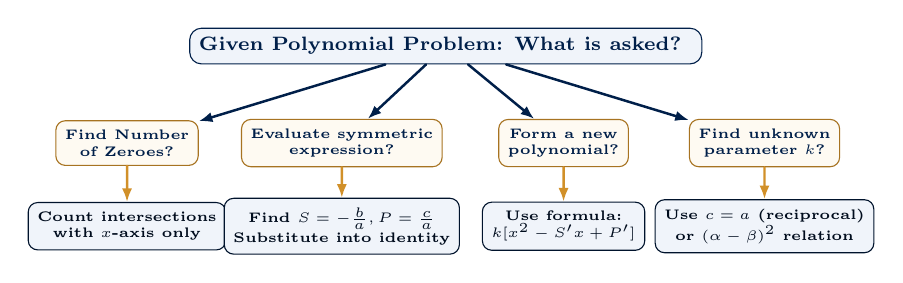
\begin{tikzpicture}[scale=0.88, line cap=round, line join=round]
  \node[draw=navy, fill=bluepale, rounded corners=1.5mm, font=\scriptsize\bfseries\color{navy}, align=center] (Start) at (0, 2.0) {
    Given Polynomial Problem: What is asked?
  };

  \node[draw=gold!80!black, fill=goldpale, rounded corners=1.2mm, font=\tiny\bfseries\color{navy}, align=center] (B1) at (-4.6, 0.6) {
    Find Number\\of Zeroes?
  };
  \node[draw=green!60!black, fill=greenpale, rounded corners=1.2mm, font=\tiny\bfseries\color{green!40!black}, align=center] (R1) at (-4.6, -0.6) {
    Count intersections\\with \textbf{$x$-axis only}
  };

  \node[draw=gold!80!black, fill=goldpale, rounded corners=1.2mm, font=\tiny\bfseries\color{navy}, align=center] (B2) at (-1.5, 0.6) {
    Evaluate symmetric\\expression?
  };
  \node[draw=green!60!black, fill=greenpale, rounded corners=1.2mm, font=\tiny\bfseries\color{green!40!black}, align=center] (R2) at (-1.5, -0.6) {
    Find $S = -\frac{b}{a}, P = \frac{c}{a}$\\
    Substitute into identity
  };

  \node[draw=gold!80!black, fill=goldpale, rounded corners=1.2mm, font=\tiny\bfseries\color{navy}, align=center] (B3) at (1.7, 0.6) {
    Form a new\\polynomial?
  };
  \node[draw=green!60!black, fill=greenpale, rounded corners=1.2mm, font=\tiny\bfseries\color{green!40!black}, align=center] (R3) at (1.7, -0.6) {
    Use formula:\\
    $k[x^2 - S'x + P']$
  };

  \node[draw=gold!80!black, fill=goldpale, rounded corners=1.2mm, font=\tiny\bfseries\color{navy}, align=center] (B4) at (4.6, 0.6) {
    Find unknown\\parameter $k$?
  };
  \node[draw=green!60!black, fill=greenpale, rounded corners=1.2mm, font=\tiny\bfseries\color{green!40!black}, align=center] (R4) at (4.6, -0.6) {
    Use $c=a$ (reciprocal)\\
    or $(\alpha-\beta)^2$ relation
  };

  \draw[-{Latex[scale=0.7]}, navy, line width=0.9pt] (Start) -- (B1);
  \draw[-{Latex[scale=0.7]}, navy, line width=0.9pt] (Start) -- (B2);
  \draw[-{Latex[scale=0.7]}, navy, line width=0.9pt] (Start) -- (B3);
  \draw[-{Latex[scale=0.7]}, navy, line width=0.9pt] (Start) -- (B4);

  \draw[-{Latex[scale=0.7]}, accent, line width=0.9pt] (B1) -- (R1);
  \draw[-{Latex[scale=0.7]}, accent, line width=0.9pt] (B2) -- (R2);
  \draw[-{Latex[scale=0.7]}, accent, line width=0.9pt] (B3) -- (R3);
  \draw[-{Latex[scale=0.7]}, accent, line width=0.9pt] (B4) -- (R4);
\end{tikzpicture}
\end{center}

\clearpage

% =============================================================================
% PAGE 12: BOARD EXAM TRAPS, VERIFICATION HACKS & PRE-SUBMISSION AUDIT
% =============================================================================
\thispagestyle{fancy}
\vspace*{0mm}

\chapterbanner{02}{EXAM TRAPS, HACKS \& PRE-SUBMISSION AUDIT}{Crucial Board Pitfalls, Instant Verification Checks \& Final Protocol}{\TrapTag}

\subhead{Module 11.1 $\vert$ Top 8 CBSE Board Exam Traps in Polynomials}

\begin{enumerate}[label=\textbf{\color{navy}\arabic*.}, leftmargin=6.5mm, itemsep=1.8pt]
  \item \textbf{Forgetting the Negative Sign in Sum of Zeroes:} $\alpha + \beta = -\frac{b}{a}$, NOT $\frac{b}{a}$. If $b = -5$, then $-\frac{b}{a} = -\frac{-5}{a} = +\frac{5}{a}$.
  \item \textbf{Omitting Multiplier $k$ in Polynomial Formation:} Writing $p(x) = x^2 - Sx + P$ without the non-zero constant $k$ loses marks when coefficients are fractional.
  \item \textbf{Counting $y$-Axis Intersections on Graphs:} Zeroes are determined \textbf{solely by intersections with the $x$-axis}. Never count the point where the curve cuts the $y$-axis!
  \item \textbf{Confusing "Number of Zeroes" with "Value of Zeroes":} If a parabola cuts the $x$-axis at $x = 3$ and $x = -2$, the \textbf{number} of zeroes is $2$, while the \textbf{values} are $3$ and $-2$.
  \item \textbf{Non-Standard Term Ordering Trap:} In polynomials like $6x^2 - 3 - 7x$, students frequently write $b = -3$ and $c = -7$. Always rearrange into standard form $ax^2 + bx + c$ ($6x^2 - 7x - 3$) first!
  \item \textbf{Incorrect Expansion of $(\alpha - \beta)^2$:} Write $(\alpha - \beta)^2 = (\alpha + \beta)^2 - 4\alpha\beta$. Do NOT confuse this with $(\alpha + \beta)^2 - 2\alpha\beta$ (which is $\alpha^2 + \beta^2$).
  \item \textbf{Attempting Long Division (Deleted Topic):} Do not use the deleted division algorithm $p(x) = g(x)q(x) + r(x)$ to solve questions. Use Vieta's formulas and symmetric identities.
  \item \textbf{Zeroes of Polynomial vs. Roots of Equation:} A polynomial has \textbf{zeroes}; an equation has \textbf{roots}. Write $p(x) = 0$ when transitioning from polynomials to equations.
\end{enumerate}

\subhead{Module 11.2 $\vert$ Algebraic Verification Hacks}
\begin{itemize}[itemsep=1.2pt]
  \item \textbf{Direct Substitution Check:} Substitute your calculated zero $\alpha$ back into $p(x)$. If $p(\alpha) \neq 0$, your root calculation is flawed.
  \item \textbf{Discriminant Reality Sanity Check:} Before looking for real zeroes, check $D = b^2 - 4ac$. If $D < 0$, no real zeroes exist.
  \item \textbf{Parity \& Sign Check:} If $c/a > 0$, both zeroes must have the \textbf{same sign}. If $c/a < 0$, zeroes must have \textbf{opposite signs}.
\end{itemize}

\subhead{Module 11.3 $\vert$ The 5-Point Pre-Submission Board Exam Audit}

\begin{center}
\small
\begin{tabularx}{\textwidth}{>{\bfseries\color{navy}}c p{44mm} X}
\toprule
\rowcolor{bluepale}Check & Verification Item & Board Evaluation Standard \\
\midrule
$\square$ 1 & Standard Form Arranged & Are terms written in strict descending powers of $x$ before reading $a, b, c$? \\
$\square$ 2 & Sign of $-\frac{b}{a}$ Verified & Did you properly apply the negative sign to $\text{Sum } = -\frac{b}{a}$? \\
$\square$ 3 & Multiplier $k$ Included & Did you write $p(x) = k[x^2 - Sx + P]$ with $k \neq 0$ stated? \\
$\square$ 4 & $x$-Axis Intersections Counted & On graph questions, did you count only $x$-axis intersections and ignore $y$-axis? \\
$\square$ 5 & Symmetric Identities Verified & Did you express symmetric expressions strictly in terms of $S$ and $P$? \\
\bottomrule
\end{tabularx}
\end{center}

\vfill
\begin{center}
  {\color{gold}\rule{0.65\textwidth}{1.2pt}}\par\vspace{2mm}
  {\Large\bfseries\color{navy}Master the Theorems. Construct the Logic. Secure the 100\%.}\par\vspace{1.5mm}
  {\small\bfseries\color{gold}MATHS MANTHAN TUITION CLASSES}\par
  {\footnotesize\color{muted}contact@mathsmanthan.co.in \quad\textbar\quad +91-8171546558 \quad\textbar\quad \url{https://mathsmanthan.co.in}}
\end{center}

\end{document}
